\chapter{Experimental Results}
\section{Experimental Setup}
The CUDA kernels are executed on NVIDIA's C1060 and C2070 GPUs. The core and memory clock frequencies of C1060 are 1.3 GHz and 800 MHz. It contains 240 cores arranged in 30 streaming multiprocessors. C2070 is Fermi-based and has core and memory clock frequencies of 1.15 GHz and 1.49 GHz. It has 448 cores arranged in fourteen streaming multiprocessors.

For our CPU executions, we use a quad-processor SMP, Xeon server. The four processors are hex-core, Intel X7460 CPUs running at 2.66GHz.

\section{Comparison with CPU}
We compare our GPU implementation with our modified NU-Minebench implementation (mentioned in Section \ref{sec:cpuMod}) running on our 24-core Xeon server. 
We use two real world datasets as input for our comparisons. 

Our first input dataset is KDD Cup 1999 \cite{kdd}. It contains 4,898,431 data points, each having 41 attributes. Tables \ref{table:kddCPU} and \ref{table:kddCPU2} show the speedup obtained with change in number of data-points and clusters respectively.

\begin{table}[htbp]
\begin{center}
\begin{tabular}{|r|p{2.8cm}|p{2.8cm}|p{2cm}|p{2.8cm}|p{2cm}|}
\hline
\multicolumn{1}{|l|}{n} & \multicolumn{1}{p{2.8cm}|}{Execution time CPU (ms)} & \multicolumn{1}{p{2.8cm}|}{Execution time C1060 (ms)} & \multicolumn{1}{p{2cm}|}{Speedup over CPU} & Execution time C2070 (ms) & \multicolumn{1}{p{2cm}|}{Speedup over CPU} \\ \hline
1000000 & 9865 & 2596 & 3.80 & 1425 & 6.92 \\ \hline
1500000 & 14672 & 3881 & 3.78 & 2117 & 6.93 \\ \hline
2000000 & 19605 & 5171 & 3.79 & 2743 & 7.15 \\ \hline
2500000 & 23828 & 6456 & 3.69 & 3414 & 6.98 \\ \hline
3000000 & 29021 & 7746 & 3.75 & 4078 & 7.12 \\ \hline
3500000 & 34075 & 9027 & 3.77 & 4688 & 7.27 \\ \hline
4000000 & 38831 & 10362 & 3.75 & 5380 & 7.22 \\ \hline
4500000 & 43605 & 11595 & 3.76 & 6036 & 7.22 \\ \hline
\end{tabular}
\end{center}
\caption{KDD Cup 1999 Data Set: Execution times for K-means on CPU and GPU. $K = 64$, $d = 41$, number of iterations$ = 50$}
\label{table:kddCPU}
\end{table}

\begin{table}[htbp]
\begin{center}
\begin{tabular}{|r|p{2.8cm}|p{2.8cm}|p{2cm}|p{2.8cm}|p{2cm}|}
\hline
\multicolumn{1}{|l|}{K} & \multicolumn{1}{p{2.8cm}|}{Execution time CPU (ms)} & \multicolumn{1}{p{2.8cm}|}{Execution time C1060 (ms)} & \multicolumn{1}{p{2cm}|}{Speedup over CPU} & Execution time C2070 (ms) & \multicolumn{1}{p{2cm}|}{Speedup over CPU} \\ \hline
32 & 10782 & 2783 & 3.87 & 1578 & 6.83 \\ \hline
64 & 19605 & 5171 & 3.79 & 2743 & 7.15 \\ \hline
96 & 28754 & 7586 & 3.79 & 3907 & 7.36 \\ \hline
128 & 37055 & 10158 & 3.65 & 5061 & 7.32 \\ \hline
160 & 46762 & 12396 & 3.77 & 6392 & 7.32 \\ \hline
\end{tabular}
\end{center}
\caption{KDD Cup 1999 Data Set: Execution times for K-means on CPU and GPU. $n = 2000000$, $d = 41$, number of iterations$ = 50$}
\label{table:kddCPU2}
\end{table}

Next we perform comparison for Covertype Data Set \cite{coverType}. It contains  581,012 data points, each having 54 attributes. Tables \ref{table:coverCPU} and \ref{table:coverCPU2} show the speedup obtained with change in number of data-points and clusters respectively.

\begin{table}[htbp]
\begin{center}
\begin{tabular}{|r|p{2.8cm}|p{2.8cm}|p{2cm}|p{2.8cm}|p{2cm}|}
\hline
\multicolumn{1}{|l|}{n} & \multicolumn{1}{p{2.8cm}|}{Execution time CPU (ms)} & \multicolumn{1}{p{2.8cm}|}{Execution time C1060 (ms)} & \multicolumn{1}{p{2cm}|}{Speedup over CPU} & Execution time C2070 (ms) & \multicolumn{1}{p{2cm}|}{Speedup over CPU} \\ \hline
100000 & 1290 & 303.4 & 4.25 & 168.5 & 7.66 \\ \hline
200000 & 2835 & 603.35 & 4.70 & 332.1 & 8.54 \\ \hline
300000 & 3227 & 889.2 & 3.63 & 494.15 & 6.53 \\ \hline
400000 & 4371 & 1186.9 & 3.68 & 652.6 & 6.70 \\ \hline
500000 & 5325 & 1472.5 & 3.62 & 817.8 & 6.51 \\ \hline
580000 & 6298 & 1710.4 & 3.68 & 954 & 6.60 \\ \hline
\end{tabular}
\end{center}
\caption{Covertype Data Set: Execution times for K-means on CPU and GPU. $K = 64$, $d = 54$, number of iterations$ = 50$.}
\label{table:coverCPU}
\end{table}

\begin{table}[htbp]
\begin{center}
\begin{tabular}{|r|p{2.8cm}|p{2.8cm}|p{2cm}|p{2.8cm}|p{2cm}|}
\hline
\multicolumn{1}{|l|}{K} & \multicolumn{1}{p{2.8cm}|}{Execution time CPU (ms)} & \multicolumn{1}{p{2.8cm}|}{Execution time C1060 (ms)} & \multicolumn{1}{p{2cm}|}{Speedup over CPU} & Execution time C2070 (ms) & \multicolumn{1}{p{2cm}|}{Speedup over CPU} \\ \hline
32 & 3145 & 761.15 & 4.13 & 476.4 & 6.60 \\ \hline
64 & 5325 & 1472.35 & 3.62 & 778.15 & 6.84 \\ \hline
96 & 7835 & 2115.2 & 3.70 & 1118.6 & 7.00 \\ \hline
128 & 10343 & 2886.55 & 3.58 & 1484.7 & 6.97 \\ \hline
160 & 12162 & 3473.4 & 3.50 & 1838.85 & 6.61 \\ \hline
192 & 15366 & 4200 & 3.66 & 2253.06 & 6.82 \\ \hline
\end{tabular}
\end{center}
\caption{Covertype Data Set: Execution times for K-means on CPU and GPU. $n = 500000$, $d = 54$, number of iterations$ = 50$.}
\label{table:coverCPU2}
\end{table}

We note that although C1060 has 240 cores, the frequency of CPU cores is twice that of GPU cores. For the case of Fermi it is in fact 2.5x times. Also, during data load intensive reduction operation, CPU has larger caches: 36 MB L2 and 64 MB L3. In comparison, C1060 does not have any L2 cache causing much larger latency for load operations during reduction.


On Fermi-based C2070 there is a 768 KB L2 cache. It enables C2070 to achieve better performance during reduction in comparison with C1060. Also, the availability of $\_\_ballot$ function ensures that the threads in a warp do not have to use shared memory for checking the membership of data points during reduction. This is why C2070 is consistently able to achieve a better speedup as compared to C2070.


\section{Comparison with Published Results}

Figure \ref{fig:kddpub} shows a comparison between our implementation and those by Li et al \cite{li_et_al}, University of Virginia \cite{che_et_al} and GPUMiner \cite{gpuminer}. The execution times are taken from \cite{li_et_al} for a sample dataset provided by KDD Cup 1999 \cite{kdd}. The sample contains 51,200 data points, each having 34 attributes. Our implementation is able to perform better than the published results in Li et al \cite{li_et_al}.

\begin{figure}[h]
	\centerline{
   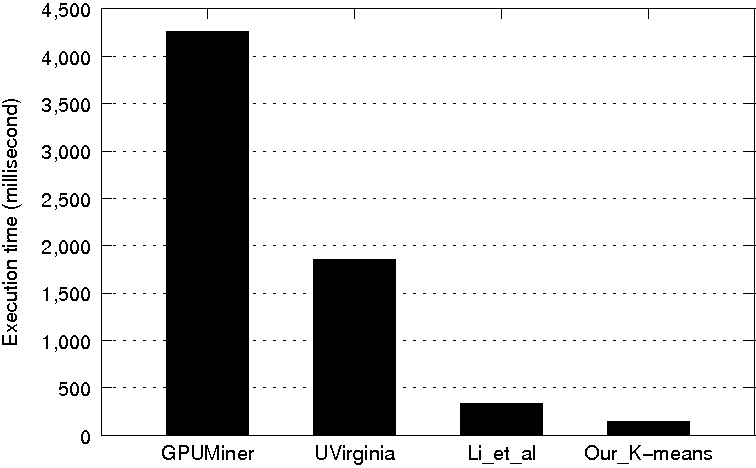
\includegraphics[width=0.8\textwidth]{./Data/comparison/kddPublished}  	
	}
	\caption{ Comparison of execution time of our implementation of K-means with Li et al \cite{li_et_al}, University of Virginia \cite{che_et_al} and GPUMiner \cite{gpuminer} for 100 iterations on KDD Cup 1999 Dataset \cite{kdd}, with $K = 32$, $d = 34$, $n = 51200$}
\label{fig:kddpub}
\end{figure}


Table \ref{table:liComp} shows a comparison of execution time of our K-means implementation with timings reported by Li et al \cite{li_et_al}. Value for $n$ is 51,200, $K$ is 32 and the execution time is taken for 100 iteration of K-means. Our K-means consistently performs better than \cite{li_et_al}. Even when $d$ = 160, we are able to achieve over 1.5x speedup.

\begin{table}[h]
\begin{center}
\begin{tabular}{|r|p{3.5cm}|p{3.5cm}|}
\hline
\multicolumn{1}{|l|}{d} & \multicolumn{1}{p{3.5cm}|}{Execution time Li et al\cite{li_et_al} (ms)} & \multicolumn{1}{p{3.5cm}|}{Execution time our K-means (ms)} \\ \hline
32 & 328 & 129 \\ \hline
64 & 403 & 185.5 \\ \hline
96 & 447 & 224.4 \\ \hline
128 & 475 & 273.3 \\ \hline
160 & 523 & 331.2 \\ \hline
\end{tabular}
\end{center}
\caption{Comparison of execution times of our K-means implementation with timings in Li et al\cite{li_et_al}. $K = 32$, $n = 51200$, number of iterations$ = 100$.}
\label{table:liComp}
\end{table}


